\section{模型建立}    
    \subsection{问题一}
        将数据导入matlab后,我们绘制出了以下图片。我们计算出每个管道的
        温度方差、平均值。总体的温度趋势表格如下
        \begin{table}[H]
            \centering
            \begin{tabular}{ p{2.5cm}|p{2.5cm}|p{2.5cm}|p{2.5cm}|p{2.5cm}  }
                \hline
                %\multicolumn{4}{|c|}{Country List} \\                                             
                0-1000&1000-2000&2000-3000&3000-4000&4000-5000\\
                \hline
                迅速向上,到达最高点后减缓&
                迅速降温,中途反弹,随后继续降温&
                继续降温直到最低点,缓慢上升一点&
                缓慢上升,中间震荡较多&
                温度趋于平稳,在区间内震荡\\
                \hline
            \end{tabular}
            \caption{趋势表}
        \end{table}

        \begin{figure}[H]
            \centering
            \begin{subfigure}{0.32\textwidth}
                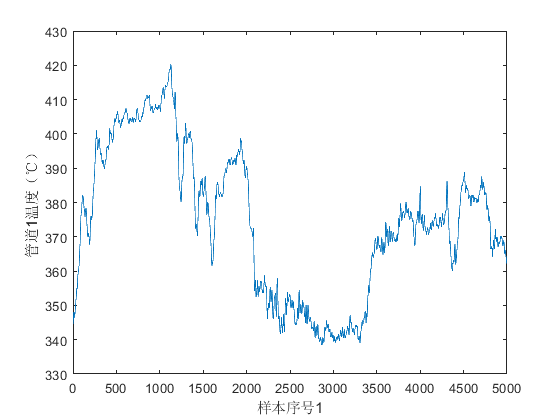
\includegraphics[width=\textwidth]{figures/p1_1.png}
                \label{p1_1}
                \caption{管一}
            \end{subfigure}
            \begin{subfigure}{0.32\textwidth}
                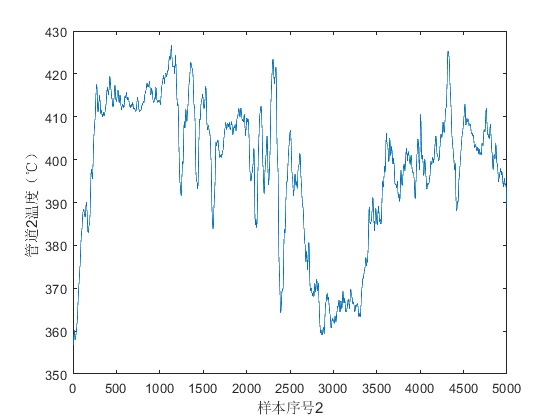
\includegraphics[width=\textwidth]{figures/p1_2.png}
                \label{p1_2}
                \caption{管二}
            \end{subfigure}
            \begin{subfigure}{0.32\textwidth}
                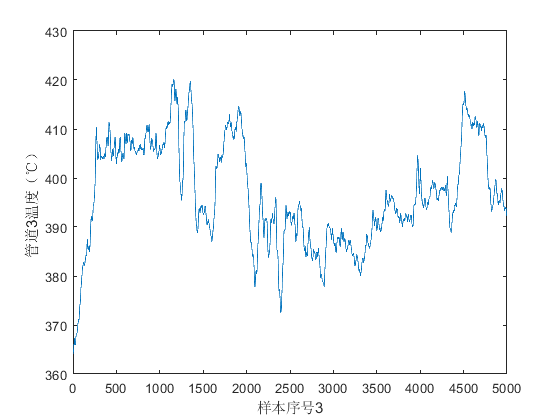
\includegraphics[width=\textwidth]{figures/p1_3.png}
                \label{p1_3}
                \caption{管三}
            \end{subfigure}
            \begin{subfigure}{0.32\textwidth}
                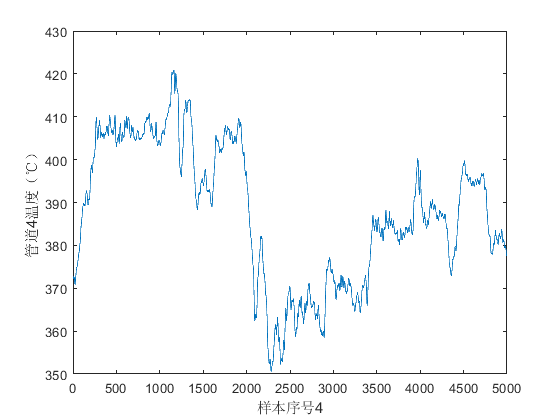
\includegraphics[width=\textwidth]{figures/p1_4.png}
                \label{p1_4}
                \caption{管四}
            \end{subfigure}
            \begin{subfigure}{0.32\textwidth}
                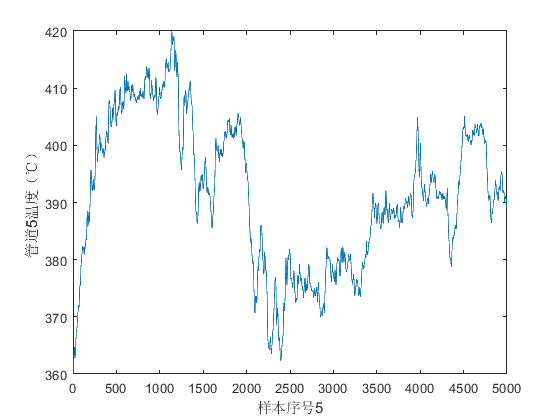
\includegraphics[width=\textwidth]{figures/p1_5.png}
                \label{p1_5}
                \caption{管五}
            \end{subfigure}
            \begin{subfigure}{0.32\textwidth}
                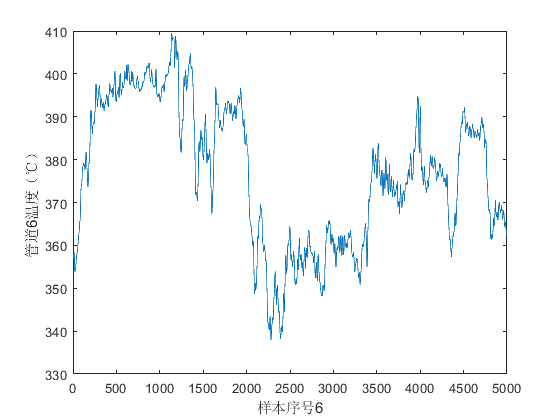
\includegraphics[width=\textwidth]{figures/p1_6.png}
                \label{p1_6}
                \caption{管六}
            \end{subfigure}
        \end{figure}

        \setcounter{figure}{0}%前面的图没有标号,这里置0包括两个图
        \begin{figure}[h]
            \centering
            \setcounter{subfigure}{6}%这里续上之前的6个小图
            \begin{subfigure}{0.24\textwidth}
                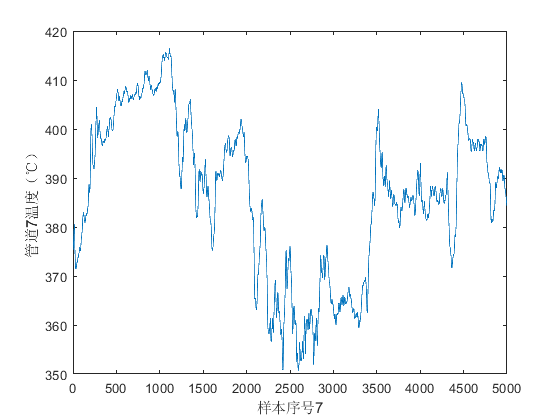
\includegraphics[width=\textwidth]{figures/p1_7.png}
                \label{p1_7}
                \caption{管七}
            \end{subfigure}
            \begin{subfigure}{0.24\textwidth}
                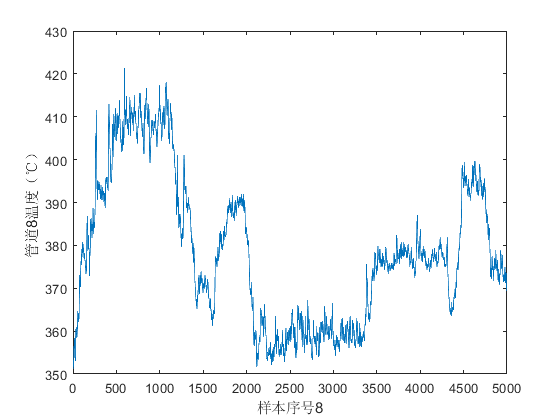
\includegraphics[width=\textwidth]{figures/p1_8.png}
                \label{p1_8}
                \caption{管八}
            \end{subfigure}
            \begin{subfigure}{0.24\textwidth}
                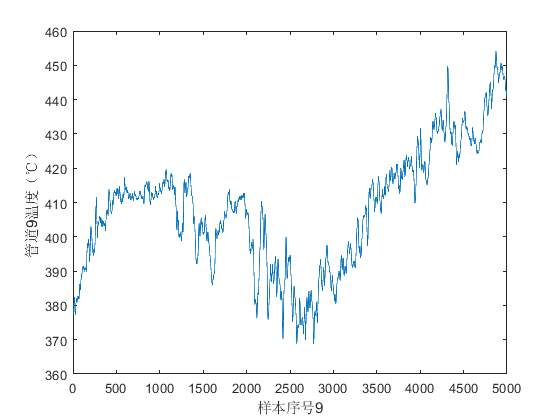
\includegraphics[width=\textwidth]{figures/p1_9.png}
                \label{p1_9}
                \caption{管九}
            \end{subfigure}
            \begin{subfigure}{0.24\textwidth}
                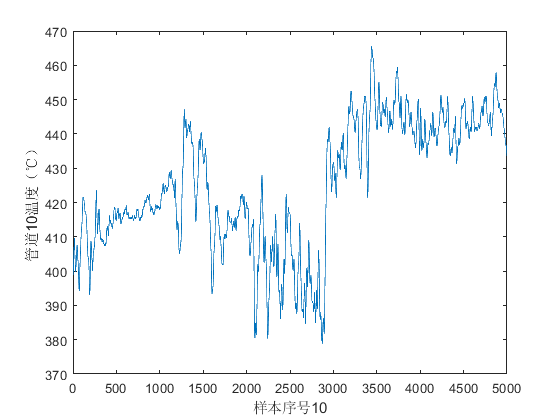
\includegraphics[width=\textwidth]{figures/p1_10.png}
                \label{p1_10}
                \caption{管十}
            \end{subfigure}
            \caption{所有的温度图}
        \end{figure}
        建立如下表格,用来具体分析,方差最值趋势
        \begin{table}[H]
            \centering
            \begin{tabular}{ c|c|c|c|c|c|c|c|c|c|c  }
                \hline
                %\multicolumn{4}{|c|}{Country List} \\                                             
                &管一&管二&管三&管四&管五&管六&管七&管八&管九&管十\\
                \hline
                方差& AF&AFG&AFG&AFG&AFG&AFG&AFG&AFG&AFG&004\\
                平均& AF&AFG&AFG&AFG&AFG&AFG&AFG&AFG&AFG&004\\
                趋势& AF&AFG&AFG&AFG&AFG&AFG&AFG&AFG&AFG&004\\
                \hline
            \end{tabular}
            \caption{管温度总览}
        \end{table}

    \subsection{问题二}
        问题二的分析。。。。
        问题二的分析。。。。
        问题二的分析。。。。
        问题二的分析。。。。
        问题二的分析。。。。

        问题二的分析。。。。问题二的分析。。。。
        问题二的分析。。。。
        问题二的分析。。。。
        问题二的分析。。。。
        问题二的分析。。。。
        问题二的分析。。。。
        问题二的分析。。。。问题二的分析。。。。
        问题二的分析。。。。

    \subsection{问题三}
        问题三的分析。。。。
    \subsection{问题四}
        问题四的分析。。。。
    \subsection{问题五}
        问题五的分析。。。。    